% ============================================================================
% Constrained Optimal Carbon Tax in a Stochastic OLG-IAM
% Deep Learning for Solving and Estimating Dynamic Models
% Duration: ~75 minutes (~35 frames)
% ============================================================================

\documentclass[aspectratio=169,11pt]{beamer}

% ---------- Theme and colors ----------
\usecolortheme{dove}
\setbeamertemplate{navigation symbols}{}
\setbeamertemplate{footline}{%
  \hfill\usebeamerfont{page number in head/foot}%
  \usebeamercolor[fg]{normal text}%
  \insertframenumber\,/\,\inserttotalframenumber\kern1em\vskip4pt}
\setbeamerfont{frametitle}{size=\huge}

% ---------- Packages ----------
\usepackage[utf8]{inputenc}
\usepackage[T1]{fontenc}
\usepackage{amsmath,amssymb,amsfonts}
\usepackage{bm}
\usepackage{graphicx}
\graphicspath{{fig/}}
\usepackage{tikz}
\usetikzlibrary{shapes,arrows.meta,positioning,calc,fit,backgrounds,patterns,decorations.pathreplacing}
\usepackage{pgfplots}
\pgfplotsset{compat=1.18}
\usepackage{booktabs}
\usepackage{hyperref}
\usepackage{multicol}
\usepackage{xcolor}

% ---------- Custom colors ----------
\definecolor{uzhblue}{rgb}{0,0,0.5}
\definecolor{uzhgreylight}{RGB}{236,238,241}
\definecolor{uzhgreydark}{RGB}{81,86,94}
\definecolor{harvardcrimson}{RGB}{153,0,0}
\definecolor{unil@blue}{RGB}{0,140,204}
\definecolor{unil@black}{RGB}{35,31,32}
\definecolor{darkgreen}{RGB}{0,100,0}
\definecolor{darkred}{RGB}{139,0,0}
\definecolor{softblue}{RGB}{70,130,180}
\definecolor{softorange}{RGB}{230,159,0}
\definecolor{softgreen}{RGB}{0,158,115}

% ---------- Set beamer colors ----------
\setbeamercolor{frametitle}{bg=uzhgreylight, fg=uzhblue}
\setbeamercolor{title}{fg=uzhblue}
\setbeamercolor{structure}{fg=uzhblue}
\setbeamercolor{block title}{bg=unil@blue, fg=white}
\setbeamercolor{block body}{bg=uzhgreylight}
\setbeamercolor{block title alerted}{bg=darkred,fg=white}
\setbeamercolor{block body alerted}{bg=red!5}
\setbeamercolor{block title example}{bg=darkgreen,fg=white}
\setbeamercolor{block body example}{bg=green!5}
\setbeamercolor{item}{fg=unil@black}
\setbeamercolor{normal text}{fg=unil@black}

% ---------- Emphasis and hyperlinks ----------
\newcommand{\emphc}[1]{\textcolor{harvardcrimson}{#1}}
\hypersetup{colorlinks,linkcolor=harvardcrimson,urlcolor=harvardcrimson}

% ---------- Math commands ----------
\newcommand{\x}{\bm{x}}
\newcommand{\X}{\bm{X}}
\newcommand{\R}{\mathbb{R}}
\newcommand{\E}[1]{\mathbb{E}\!\left[#1\right]}
\newcommand{\nn}{\mathcal{N}_{\bm{\rho}}}
\DeclareMathOperator*{\argmin}{arg\,min}
\DeclareMathOperator*{\argmax}{arg\,max}
\DeclareMathOperator{\Var}{Var}

% ---------- Title ----------
\title[Deep Learning for Dynamic Economic Models]
{Deep Learning for Economics and Finance}
\subtitle{Stochastic IAMs with DEQNs, GP surrogates, Sobol/Shapley, constrained Pareto-improving carbon-tax design}
\author{Simon Scheidegger}
\institute[HEC Lausanne]{HEC, University of Lausanne}
\date{}

\begin{document}
% --- Exercise pause badge ---
\newcommand{\exercisepause}{%
  \tikz[baseline=(X.base)]{\node[fill=darkgreen!80!black, text=white,
  rounded corners=2pt, inner sep=3pt, font=\scriptsize\bfseries](X){PAUSE --- 5 min};}}


% ============================================================================
% SECTION 0: TITLE & ROADMAP
% ============================================================================

% --- Frame 1: Title ---
{\setbeamercolor{background canvas}{bg=uzhgreylight}
\begin{frame}
\titlepage
\vspace{-0.4cm}
\begin{center}
{\footnotesize Based on: K\"ubler, Scheidegger, Surbek (2025, arXiv:2507.01704)}\\[2pt]
{\footnotesize Reading: \texttt{JPE\_Macro.pdf}; public draft: arXiv:2507.01704}\\[4pt]
{\footnotesize Materials: \url{https://github.com/sischei/Deep_Learning_for_Solving_And_Estimating_Dynamic_Economic_Models}}
\end{center}
\end{frame}
}

% --- Frame 2: Outline ---
\begin{frame}{Outline of This Lecture}
\begin{columns}[T]
\column{0.48\textwidth}
\textbf{Part I: Motivation}
\begin{itemize}
    \item Why OLG for climate policy?
    \item Winners and losers from carbon taxation
    \item Our contribution and the 3-step method
\end{itemize}

\vspace{0.4em}
\textbf{Part II: The OLG-IAM Model}
\begin{itemize}
    \item Technology, households, climate
    \item Carbon tax and transfers
    \item The planner's problem
\end{itemize}

\column{0.48\textwidth}
\textbf{Part III: Full Derivation}
\begin{itemize}
    \item Firm FOCs, household Euler equations
    \item Market clearing and equilibrium system
    \item Nonstationarity and time as state variable
\end{itemize}

\vspace{0.4em}
\textbf{Part IV: 3-Step Pipeline}

\textbf{Part V: Results}

\vspace{0.4em}
\begin{alertblock}{Bridge from Lecture 08}
From RA $\rightarrow$ \emphc{heterogeneous agents} (OLG) and UQ $\rightarrow$ \emphc{optimal policy search}.
\end{alertblock}
\end{columns}
\end{frame}

% --- Learning objectives ---
\begin{frame}{Learning objectives}
\textbf{By the end of this lecture you should be able to:}
\begin{itemize}
  \item Formulate constrained optimal-policy problems in heterogeneous-agent OLG-IAM models
  \item Train a DEQN with pseudo-states covering both economic controls and policy parameters
  \item Build welfare surrogates and solve for Pareto-improving carbon-tax rules
  \item Diagnose intergenerational trade-offs and tail-risk insurance mechanisms in policy design
  \item Compare linear implementable rules against unconstrained optima with quantified welfare losses
\end{itemize}
\end{frame}


% ============================================================================
% SECTION I: MOTIVATION
% ============================================================================
\section{Motivation --- Optimal Policy with Heterogeneous Agents}

% --- Frame 3: Section Divider ---
\begin{frame}{}
\vfill
\begin{center}
{\Huge \textcolor{uzhblue}{\textbf{Part I}}}\\[12pt]
{\LARGE Optimal Policy with Heterogeneous Agents}
\end{center}
\vfill
\end{frame}

% --- Frame 4: The challenge ---
\begin{frame}{The Challenge: Climate Risk and Heterogeneity}
\begin{figure}
    \centering
    
\includegraphics[width=0.49\linewidth]{olg_agents.jpg}
    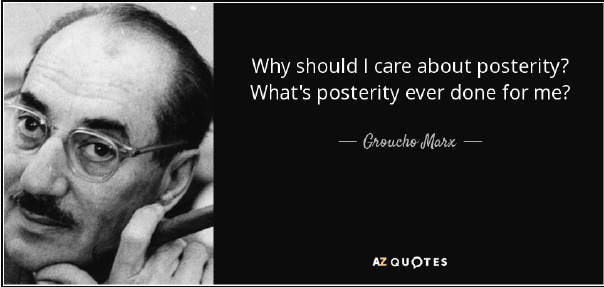
\includegraphics[width=0.49\linewidth]{quote.png}
\end{figure}

\vspace{-0.1cm}
\small
\begin{itemize}
    \item Current research in climate change macro often resorts to \textcolor{blue}{simplifying assumptions} (e.g., representative agent) or searches for Pareto improvements by \textcolor{blue}{guessing}.
    \item We need tools for optimal policy within \textcolor{blue}{globally solved} models that take into account \textcolor{blue}{heterogeneity and stochasticity}.
\end{itemize}
\end{frame}

% --- Frame 5: Why OLG ---
\begin{frame}{Why Overlapping Generations (OLG)?}
\begin{itemize}
    \setlength\itemsep{1em}
    \item \textbf{Intergenerational equity}: Climate policy creates winners and losers across generations.
    \item \textbf{Political feasibility}: Current cohorts bear costs; future cohorts reap benefits.
    \item \textbf{No representative agent}: With OLG, there is no single welfare function --- must aggregate across cohorts.
    \item \textbf{Pareto constraint}: A policy that improves aggregate welfare but hurts current generations may be politically infeasible.
\end{itemize}

\vspace{0.2cm}
\begin{alertblock}{Key question}
Can we find carbon tax rules that are \emphc{Pareto-improving} --- i.e., no generation is worse off?
\end{alertblock}
\end{frame}

% --- Frame 6: Our contribution ---
\begin{frame}{Our Contribution: A Scalable Policy Framework}
\begin{columns}[t]
\begin{column}{0.50\textwidth}
    \textbf{The Method}

    \vspace{0.3em}
    \centering
    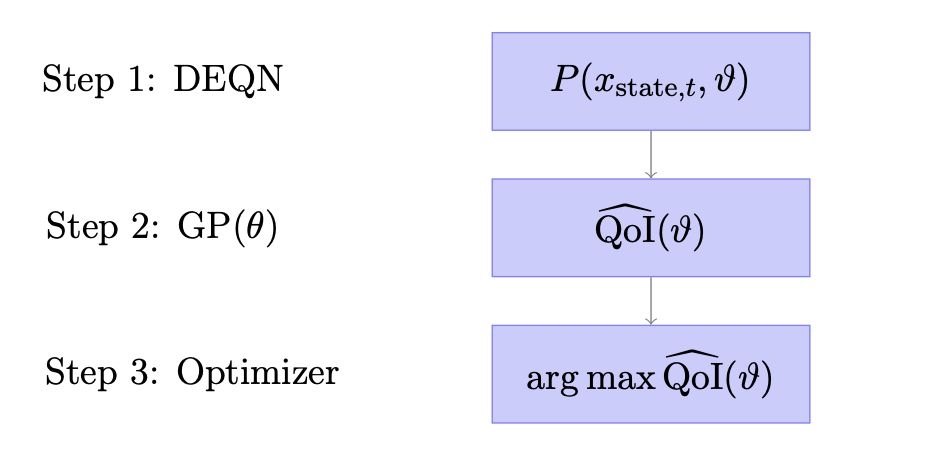
\includegraphics[width=0.92\linewidth]{flow_chart_2.png}

    \vspace{0.3em}
    \raggedright
    \small A 3-step ML pipeline to alleviate the \textcolor{blue}{curse of dimensionality}.
\end{column}

\begin{column}{0.50\textwidth}
    \textbf{The Application}

    \vspace{0.2em}
    \small
    We compute the first \textcolor{blue}{globally optimal, Pareto-improving carbon tax} in a stochastic OLG model with tipping points.

    \vspace{1.0em}
    \textbf{A Generic Blueprint}

    \vspace{0.2em}
    A universal framework for \textbf{almost any} stochastic heterogeneous-agent model: \textcolor{blue}{solve global equilibria} and derive \textcolor{blue}{constrained-optimal policies}.
\end{column}
\end{columns}
\end{frame}

% --- Frame 7: 3-step overview ---
\begin{frame}{The 3-Step Method Overview}
\begin{center}
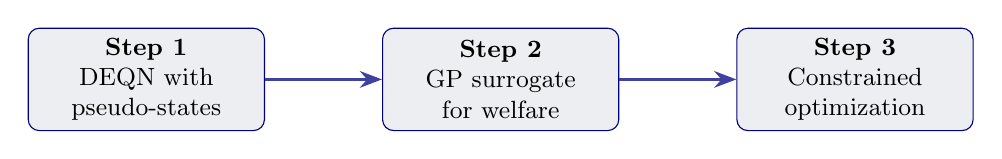
\begin{tikzpicture}[
    box/.style={rectangle, draw=uzhblue, fill=uzhgreylight, rounded corners=4pt,
                minimum width=3cm, minimum height=1.3cm, align=center, font=\small},
    arr/.style={-{Stealth[length=2.8mm]}, very thick, uzhblue!75}
]
\node[box] (deqn) at (0,0) {\textbf{Step 1}\\DEQN with\\pseudo-states};
\node[box] (gp) at (4.5,0) {\textbf{Step 2}\\GP surrogate\\for welfare};
\node[box] (opt) at (9,0) {\textbf{Step 3}\\Constrained\\optimization};

\draw[arr] (deqn) -- (gp);
\draw[arr] (gp) -- (opt);
\end{tikzpicture}
\end{center}

\vspace{0.3cm}
\begin{itemize}
    \item \textbf{Step 1}: Solve the OLG equilibrium globally for \emphc{all} tax rules at once (pseudo-states).
    \item \textbf{Step 2}: Build a GP surrogate mapping tax parameters $\rightarrow$ welfare.
    \item \textbf{Step 3}: Find optimal tax-transfer rule subject to Pareto constraints.
\end{itemize}
\end{frame}

% ============================================================================
% SECTION II: THE STOCHASTIC OLG-IAM MODEL
% ============================================================================
\section{The Stochastic OLG-IAM Model}

% --- Frame 8: Section Divider ---
\begin{frame}{}
\vfill
\begin{center}
{\Huge \textcolor{uzhblue}{\textbf{Part II}}}\\[12pt]
{\LARGE The Stochastic OLG-IAM Model}
\end{center}
\vfill
\end{frame}

% --- Frame 9: Model overview ---
\begin{frame}{Model Overview}
\begin{itemize}
    \setlength\itemsep{0.8em}
    \item \textbf{12 overlapping generations} of selfish agents.
    \item \textbf{5-year periods}: agents live from age 20 to age 80.
    \item Use a \textbf{simple climate module} (Dietz and Venmans, 2019): cumulative emissions $\rightarrow$ temperature.
    \item Use a \textbf{damage function with stochastic tipping} (Kotlikoff et al., 2021).
    \item \textbf{Exogenously declining carbon intensity} as in DICE-2016 (Nordhaus, 2017).
    \item Carbon tax revenues recycled through \textbf{parameterized transfer rules}.
\end{itemize}
\end{frame}

% --- Frame 10: Technology / Firms ---
\begin{frame}{Technology / Firms}
\small
Firms produce \textcolor{blue}{final output $Y_t$ and emissions $e_t$} with capital $K_t$ and labor $L_t$, choosing abatement $\mu_t$:
\begin{equation*}
(Y_t,\; e_t) = \Big(\Omega_t(T_t)\Phi(\mu_t) K_t^\alpha L_t^{1-\alpha} + (1-\delta)K_t,\;\; \kappa_t(1-\mu_t)K_t^\alpha L_t^{1-\alpha}\Big)
\end{equation*}

\begin{itemize}
    \item $\Omega_t(T_t)$: retained-output factor after climate damages
    \item $\Phi(\mu_t) = 1 - \theta_1 \mu_t^{\theta_2}$: net-of-abatement-cost factor
    \item $\kappa_t$: carbon intensity (declines stochastically over time)
\end{itemize}

\vspace{0.2cm}
\textbf{Profit maximization} with carbon tax $\tau_t$:
\[
\max_{\mu_t, K_t, L_t} \;\; \Omega_t(T_t)(1-\theta_1 \mu_t^{\theta_2})K_t^\alpha L_t^{1-\alpha} + (1-\delta)K_t - w_t L_t - (1+r_t)K_t - \tau_t(1-\mu_t)\kappa_t K_t^\alpha L_t^{1-\alpha}
\]
subject to $0 \leq \mu_t \leq 1$.
\end{frame}

% --- Frame 11: Households ---
\begin{frame}{Households}
\small
Agents enter the labor force at age 20 with 0 assets and die at age 80 (12 periods).

\vspace{0.2cm}
\textbf{Lifetime utility:}
\[
\mathbb{E}_t \sum_{j=1}^{12} \beta^{j-1} \frac{C_{t+j-1,j}^{1-\sigma_u}}{1-\sigma_u}
\]

\textbf{Budget constraint:}
\[
C_{t,j} + a_{t+1,j+1} = (1+r_t) a_{t,j} + w_t l_j + \mathbb{T}_{t,j}
\]

\begin{itemize}
    \item $C_{t,j}$, $a_{t,j}$, $l_j$, $\mathbb{T}_{t,j}$: consumption, assets, labor endowment, transfer of generation born at $t$, age $j$
    \item Agents work for 8 periods, then retire (ages 9--12: 40\% labor as pension proxy)
    \item $\beta$: discount factor, $\sigma_u$: coefficient of relative risk aversion
\end{itemize}

\vspace{0.2cm}
\textbf{Welfare criterion:} $U_t = \mathbb{E}_0 \sum_{j=1}^{12} \beta^{j-1} \frac{C_{t+j-1,j}^{1-\sigma_u}}{1-\sigma_u}$; \; use $\tilde{U}_t$ under taxation.
\end{frame}

% --- Frame 12: Carbon tax and transfers ---
\begin{frame}{Carbon Tax and Transfer Schemes}
\small
\begin{itemize}
    \item Tax $\tau_t$ on emissions; revenue redistributed to currently alive agents each period.
    \item Transfer schemes may create \emphc{winners and losers} (Kotlikoff et al., 2021).
\end{itemize}

\vspace{0.2cm}
\textbf{Two transfer policies:}
\begin{enumerate}
    \item \textcolor{blue}{``10\% declining scheme''}: youngest generation gets the highest share, each older generation gets 10\% less:
    \[
    \mathbb{T}_{t,j} = 0.9^{(j-1)} \cdot 0.1394 \cdot \tau_t e_t, \quad j \in \{2, \ldots, 12\}
    \]
    \item \textcolor{blue}{``Optimal transfers''}: transfer shares to each generation are \emphc{optimized} (fixed at $t=0$).
\end{enumerate}

\vspace{0.2cm}
Normalization: shares sum to 1.
\end{frame}

% --- Frame 13: Climate module ---
\begin{frame}{Climate Module: Cumulative Emissions $\rightarrow$ Temperature}
\small
\begin{columns}[T]
\column{0.55\textwidth}
Climate science shows a near-linear link between cumulative CO$_2$ emissions and temperature:
\[
T^{\mathrm{AT}}_t \approx \sigma_{\mathrm{CCR}} \sum_{s=0}^t E_s
\]
where $\sigma_{\mathrm{CCR}}$ is the Carbon-Climate Response (TCRE), ranging from 1.0$^\circ$C to 2.3$^\circ$C per 1000 GtC.

\vspace{0.2cm}
\textbf{Damage function with stochastic tipping:}
\[
\Omega_t(T_t) = \frac{1}{1 + \left(\frac{1}{\psi_1} T_t\right)^2 + \left(\frac{1}{2 \cdot TP_t} T_t\right)^{6.754}}
\]
$TP_t$ follows a truncated random walk in $[2.5, 3.5]$.

\column{0.42\textwidth}
\textbf{Stochastic shocks:}
\begin{itemize}
    \item $\kappa_t$: AR(1) with time-varying persistence
    \[
    \kappa_t = \rho_t \kappa_{t-1} + \epsilon_{\kappa,t}
    \]
    $\rho_t = \rho_0 + (\rho_\infty - \rho_0)(1-e^{-\delta^\rho 5t})$

    \item $TP_t$: random walk
    \[
    TP_t = TP_{t-1} + \epsilon_{TP,t}
    \]
    \item Both shocks: 3-point discretization
\end{itemize}
\end{columns}
\end{frame}

% --- Finger Exercise: Social Cost of Carbon ---
\begin{frame}{\exercisepause{} Finger Exercise: Interpreting the Social Cost of Carbon}
\begin{exampleblock}{Exercise}
Suppose the damage-loss function is $D(T) = 1 - \frac{1}{1 + \pi_1 T^2}$ with $\pi_1 = 0.00236$ and current warming $T = 1.1^\circ\mathrm{C}$.
\begin{enumerate}
    \item Compute the current output loss $D(1.1)$ as a percentage of GDP.
    \item If global GDP is \$100 trillion, what is the annual damage in dollars?
    \item The SCC is defined as the present-value damage from one additional ton of CO$_2$. If the SCC is \$50/tCO$_2$: should a firm that can abate at \$30/tCO$_2$ do so?  What about at \$80/tCO$_2$?
\end{enumerate}
\end{exampleblock}
\end{frame}

\begin{frame}{Solution: Interpreting the Social Cost of Carbon}
\begin{block}{Answer}
\begin{enumerate}
    \item $D(1.1) = 1 - \frac{1}{1 + 0.00236 \times 1.21} = 1 - \frac{1}{1.002856} \approx 0.00285 = 0.285\%$ of GDP.
    \item $0.00285 \times 100\text{ trillion} \approx \$285$ billion per year.
    \item Abate at \$30/tCO$_2$: \emphc{yes}---the cost (\$30) is below the social benefit (\$50).  At \$80/tCO$_2$: \emphc{no}---the cost exceeds the benefit.  The SCC is the \emphc{optimal carbon tax}: abate all sources cheaper than SCC, leave the rest.
\end{enumerate}
\end{block}
\end{frame}

% --- Frame 14: The planner's problem ---
\begin{frame}{The Planner's Problem}
\footnotesize
\textbf{Objective:} Choose policy parameters $\vartheta$ (taxes \& transfers) to maximize social welfare:
\[
\max_\vartheta \;\; \mathcal{W}(\vartheta) = \sum_{t=-10}^{30} \gamma_t \tilde{U}_t(\vartheta) \quad \text{s.t.} \quad \tilde{U}_t(\vartheta) \geq U_t \;\; \forall t \;\; \text{(if Pareto constrained)}
\]

\textbf{Welfare metric:} Consumption equivalence factor
\[
\mathrm{CE}_t = \left(\frac{\tilde{U}_t}{U_t}\right)^{\frac{1}{1-\sigma_u}} - 1 \qquad \text{(where $U_t$ is BAU utility)}
\]

\textbf{Scope:}
\begin{itemize}\itemsep0pt
    \item Horizon: 40 generations (11 current, 29 future).
    \item Complexity: high-dimensional $\vartheta$ in a stochastic setting.
    \item Pareto constraint: every cohort weakly better off than under BAU.
    \item Generation weights $\gamma_t = 1$ (utilitarian; Negishi or discounted weights also admissible).
\end{itemize}
\end{frame}

% ============================================================================
% SECTION III: FULL DERIVATION --- EQUILIBRIUM CONDITIONS
% ============================================================================
\section{Full Derivation --- Equilibrium Conditions}

% --- Frame 15: Section Divider ---
\begin{frame}{}
\vfill
\begin{center}
{\Huge \textcolor{uzhblue}{\textbf{Part III}}}\\[12pt]
{\LARGE Full Derivation --- Equilibrium Conditions}
\end{center}
\vfill
\end{frame}

% --- Frame 16: Firm's optimization ---
\begin{frame}{Firm's Optimization Problem}
\small
Firms maximize profits given a carbon tax $\tau_t$:
\[
\max_{\mu_t, K_t, L_t} \;\; \Omega_t(T_t)(1-\theta_1 \mu_t^{\theta_2})K_t^\alpha L_t^{1-\alpha} + (1-\delta)K_t - w_t L_t - (1+r_t)K_t - \tau_t(1-\mu_t)\kappa_t K_t^\alpha L_t^{1-\alpha}
\]
subject to $0 \leq \mu_t \leq 1$.

\vspace{0.2cm}
\textbf{Interpretation:}
\begin{itemize}
    \item Output net of damages and abatement costs
    \item Minus factor payments (wages, rental rate)
    \item Minus carbon tax on unabated emissions
\end{itemize}
\end{frame}

% --- Frame 17: Firm FOCs ---
\begin{frame}{Derivation: Firm First-Order Conditions}
\small
\textbf{w.r.t.\ $\mu_t$} (marginal abatement cost = tax):
\[
\tau_t \kappa_t = \Omega_t(T_{\mathrm{AT},t})\, \theta_1 \theta_2\, \mu_t^{\theta_2 - 1}
\]

\textbf{w.r.t.\ $K_t$} (rental rate of capital):
\begin{align*}
r_t &= \Big[\Omega_t(T_{\mathrm{AT},t})(1-\theta_1 \mu_t^{\theta_2}) - \tau_t \kappa_t(1-\mu_t)\Big]\, \alpha K_t^{\alpha-1} L_t^{1-\alpha} - \delta
\end{align*}

\textbf{w.r.t.\ $L_t$} (wage rate):
\begin{align*}
w_t &= \Big[\Omega_t(T_{\mathrm{AT},t})(1-\theta_1 \mu_t^{\theta_2}) - \tau_t \kappa_t(1-\mu_t)\Big]\, (1-\alpha) K_t^\alpha L_t^{-\alpha}
\end{align*}

\vspace{0.2cm}
\begin{exampleblock}{Intuition}
\begin{itemize}
    \item Abatement FOC: firm abates up to the point where marginal cost equals the tax
    \item Factor prices: net of both damage \emphc{and} tax wedge on emissions
\end{itemize}
\end{exampleblock}
\end{frame}

% --- Frame 18: Household optimization ---
\begin{frame}{Household's Optimization Problem}
\small
Household born at time $t$ solves:
\[
\max_{\{C_{t+j-1,j},\, a_{t+j,j+1}\}_{j=1}^{12}} \;\; \mathbb{E}_t \sum_{j=1}^{12} \beta^{j-1} \frac{C_{t+j-1,j}^{1-\sigma_u}}{1-\sigma_u}
\]

\textbf{Subject to:}
\[
C_{t,j} + a_{t+1,j+1} = (1+r_t) a_{t,j} + w_t l_j + \mathbb{T}_{t,j} \qquad \forall j = 1, \ldots, 12
\]

\textbf{Boundary conditions:}
\[
a_{t,1} = 0 \qquad \text{(born with no assets)}, \qquad a_{t+1,12} = 0 \qquad \text{(no bequest)}
\]

\vspace{0.2cm}
Write the Lagrangian with multipliers $\lambda_{t,j}$ for each period's budget constraint.
\end{frame}

% --- Frame 19: Household Euler equation ---
\begin{frame}{Derivation: Household Euler Equation}
\small
\textbf{FOC w.r.t.\ $C_{t,j}$:}
\[
\beta^{j-1} C_{t,j}^{-\sigma_u} = \lambda_{t,j}
\]

\textbf{FOC w.r.t.\ $a_{t+1,j+1}$:}
\[
\lambda_{t,j} = \mathbb{E}_t\left[(1+r_{t+1})\lambda_{t+1,j+1}\right]
\]

\textbf{Combining --- the Euler equation:}
\[
\boxed{C_{t,j}^{-\sigma_u} = \beta\, \mathbb{E}_t\!\left[(1+r_{t+1})\, C_{t+1,j+1}^{-\sigma_u}\right] \qquad \forall j = 1, \ldots, 11}
\]

\textbf{Plus budget constraint:}
\[
C_{t,j} + a_{t+1,j+1} = (1+r_t) a_{t,j} + w_t l_j + \mathbb{T}_{t,j}
\]

\vspace{0.1cm}
\begin{alertblock}{Note}
11 Euler equations + 12 budget constraints + 2 boundary conditions per cohort.
\end{alertblock}
\end{frame}

% --- Frame 20: Market clearing ---
\begin{frame}{Market Clearing Conditions}
\small
\textbf{Capital market:}
\[
\sum_{j=1}^{12} a_{t,j} = K_t \qquad \forall t
\]

\textbf{Labor market:}
\[
\sum_{j=1}^{12} l_j = L_t \qquad \forall t
\]

\textbf{Government budget (tax revenue = transfers):}
\[
\sum_{j=1}^{12} \mathbb{T}_{t,j} = \tau_t\, e_t \qquad \forall t
\]

\vspace{0.2cm}
\begin{exampleblock}{Complete system}
Firm FOCs + household Euler equations + market clearing + climate laws of motion $=$ full equilibrium.
\end{exampleblock}
\end{frame}

% --- Frame 21: KEY SLIDE --- Nonstationarity reprise ---
\begin{frame}{Nonstationarity and Time as State Variable (Reprise)}
\begin{alertblock}{Same lesson as Lecture 08 --- now in OLG}
The OLG-IAM is \emphc{nonstationary}: carbon intensity $\kappa_t$, abatement cost $\theta_{1,t}$, population, and TFP are all time-indexed exogenous sequences.
\end{alertblock}

\vspace{0.2cm}
\textbf{Specifics:}
\begin{itemize}
    \item $\kappa_t$: AR(1) with time-dependent coefficient $\rho_t = \rho_0 + (\rho_\infty - \rho_0)(1-\exp(-\delta^\rho \cdot 5t))$
    \item Abatement cost $\theta_{1,t}$ declines over time
    \item Population and TFP are exogenous sequences
\end{itemize}

\vspace{0.2cm}
\textbf{State vector:}
\[
\x = \Big[\underbrace{\emphc{t},\; TP_t,\; TP_{\mathrm{reached}},\; \kappa_t,\; E_t}_{5 \text{ non-asset states}},\; \underbrace{a_{t,j}}_{12 \text{ assets}},\; \textcolor{blue}{\vartheta}\Big] \in \mathbb{R}^{12 + 5 + d_\vartheta}
\]

\vspace{0.1cm}
Time enters the neural net as an input --- the policy function is $\nn(t, \text{states}, \text{params})$.
\end{frame}

% --- Frame 22: Equilibrium system summary ---
\begin{frame}{Complete Equilibrium System Summary}
\tiny
\begin{columns}[T]
\column{0.48\textwidth}
\textbf{Firm FOCs:}
\begin{align*}
0 &= \tau_t \kappa_t - \Omega_t \theta_1 \theta_2 \mu_t^{\theta_2-1} \tag{$\mu_t$} \\
r_t &= [\Omega_t(1-\theta_1 \mu_t^{\theta_2}) \\
    &\quad - \tau_t \kappa_t(1-\mu_t)]\alpha K_t^{\alpha-1}L_t^{1-\alpha} - \delta \tag{$K_t$} \\
w_t &= [\Omega_t(1-\theta_1 \mu_t^{\theta_2}) \\
    &\quad - \tau_t \kappa_t(1-\mu_t)](1-\alpha)K_t^\alpha L_t^{-\alpha} \tag{$L_t$}
\end{align*}

\textbf{Household Euler equations:}\\
For all $j = 1, \ldots, 11$:
\begin{align*}
C_{t,j}^{-\sigma_u} &= \beta\, \mathbb{E}_t[(1+r_{t+1})C_{t+1,j+1}^{-\sigma_u}] \tag{EE} \\
C_{t,j} + a_{t+1,j+1} &= (1+r_t)a_{t,j} + w_t l_j + \mathbb{T}_{t,j} \tag{BC}
\end{align*}

\column{0.48\textwidth}
\textbf{Market clearing:}
\begin{align*}
K_t &= \sum_{j=1}^{12} a_{t,j} \tag{$K$} \\
L_t &= \sum_{j=1}^{12} l_j \tag{$L$} \\
\tau_t e_t &= \sum_{j=1}^{12} \mathbb{T}_{t,j} \tag{$\mathbb{T}$}
\end{align*}

\textbf{Climate:}
\begin{align*}
T^{\mathrm{AT}}_t &= \sigma_{\mathrm{CCR}} \sum_{s=0}^t E_s \\
E_t &= E_{t-1} + \kappa_t(1-\mu_t)K_t^\alpha L_t^{1-\alpha}
\end{align*}

\textbf{Stochastic dynamics:}
\begin{align*}
\kappa_t &= \rho_t \kappa_{t-1} + \epsilon_{\kappa,t} \\
TP_t &= TP_{t-1} + \epsilon_{TP,t}
\end{align*}
\end{columns}
\end{frame}

% --- Frame 23: From equilibrium to DEQN ---
\begin{frame}{From Equilibrium Conditions $\rightarrow$ DEQN Residuals}
\small
Each equation becomes a residual $G_i$; loss $= \sum_i G_i^2$.

\vspace{0.2cm}
\textbf{Network inputs (state vector):}
\[
\x = [t,\; TP_t,\; TP_{\mathrm{reached}},\; \kappa_t,\; E_t,\; a_{t,j},\; \textcolor{blue}{\vartheta}] \in \mathbb{R}^{12 + 5 + d_\vartheta}
\]

\textbf{Network outputs (policy vector):}
\[
y = [a_{t+1,j+1},\; v_{t,j}] \in \mathbb{R}^{2(A-1)} = \mathbb{R}^{22}
\]

\vspace{0.2cm}
\begin{columns}[T]
\column{0.49\textwidth}
\textbf{Why include $\vartheta$?}
\begin{itemize}
    \item Tax rule parameters $\tau(\vartheta)$
    \item Transfer shares as pseudo-states
    \item DEQN learns policies for \emphc{all} tax rules and transfers at once
\end{itemize}

\column{0.49\textwidth}
\textbf{Diagnostics to report:}
\begin{itemize}
    \item Runtime and hardware configuration
    \item Residual MSE and Euler-error distribution
    \item Robustness to seeds and stress states
\end{itemize}
\end{columns}
\end{frame}

% ============================================================================
% SECTION IV: THE 3-STEP SOLUTION PIPELINE
% ============================================================================
\section{The 3-Step Solution Pipeline}

% --- Frame 24: Section Divider ---
\begin{frame}{}
\vfill
\begin{center}
{\Huge \textcolor{uzhblue}{\textbf{Part IV}}}\\[12pt]
{\LARGE The 3-Step Solution Pipeline}
\end{center}
\vfill
\end{frame}

% --- Frame 25: Step 1 ---
\begin{frame}{Step 1: DEQN with Pseudo-States}
\footnotesize
\begin{itemize}
    \item Include tax parameters $\vartheta = (\vartheta_0, \vartheta_E, \vartheta_\kappa, \vartheta_{TP})$ + 11 transfer shares as pseudo-states.
    \item DEQN learns the equilibrium for \emphc{all} tax rules at once.
\end{itemize}

\vspace{0.05cm}
\begin{center}
\scriptsize
\begin{tabular}{ll}
\toprule
\textbf{Hyperparameter} & \textbf{Value} \\
\midrule
Hidden layers & 2 \\
Units per layer & 256 \\
Activation & GeLU \\
Optimizer (LR) & Adam ($10^{-5}$) \\
Batch size & 64 \\
Inputs & $12 + 5 + d_\vartheta$ \\
Outputs & $2 \times (A-1) = 22$ \\
Sim.\ episode length & 70 steps ($\times$ 5y = 350y) \\
\bottomrule
\end{tabular}
\end{center}

\vspace{0.05cm}
\begin{exampleblock}{Key advantage over brute-force}
Pseudo-states replace many separate tax-rule solves with one amortized equilibrium solve.
\end{exampleblock}
\end{frame}

% --- Frame 26: Step 2 ---
\begin{frame}{Step 2: GP Surrogate for Welfare}
\small
\textbf{Map $\vartheta \rightarrow \mathbb{E}[\mathcal{W}(\vartheta)]$ via Gaussian Process:}
\begin{itemize}
    \item 450 LHS points + 50 BAL points = 500 total design points
    \item Leave-one-out error $\sim 10^{-4}$
    \item Two targets:
    \begin{enumerate}
        \item Aggregate welfare scalar $\mathcal{W}(\vartheta)$
        \item Vector of 40 cohort utilities $\tilde{U}_t(\vartheta)$ (for Pareto constraints)
    \end{enumerate}
\end{itemize}

\vspace{0.2cm}
\begin{block}{Why a surrogate?}
\begin{itemize}
    \item Each DEQN simulation is fast ($\sim$ seconds), but evaluating thousands of $\vartheta$ for optimization is still expensive.
    \item GP provides \emphc{predictive uncertainty} $\rightarrow$ guides BAL acquisition.
    \item 21st-century lookup table: Welfare($\vartheta_1, \ldots, \vartheta_N$).
\end{itemize}
\end{block}
\end{frame}

% --- Frame 27: Step 3 ---
\begin{frame}{Step 3: Constrained Optimization}
\small
\textbf{Find optimal tax-transfer rule:}
\[
\vartheta^* = \argmax_\vartheta \; \mathcal{W}(\vartheta) \qquad \text{s.t.} \quad \tilde{U}_t(\vartheta) \geq U_t \;\; \forall t
\]

\begin{itemize}
    \item Linear constraints on tax function staying in feasible range
    \item Pareto constraints ensure no generation is worse off
    \item Optimization runs on the \emphc{GP surrogate} (milliseconds per evaluation)
\end{itemize}

\vspace{0.2cm}
\begin{alertblock}{Computational savings}
Full constrained policy search in minutes, not days/weeks.
\end{alertblock}
\end{frame}

% --- Frame 28: Three policy scenarios ---
\begin{frame}{Three Policy Scenarios}
\small
\begin{enumerate}
    \setlength\itemsep{0.8em}
    \item \textbf{Scenario 1: Unconstrained welfare max with exogenous transfers}
    \begin{itemize}
        \item Tax rule: $\tau_t(E_t) = \vartheta_0 + \vartheta_E \cdot E_t$
        \item 10\% declining transfer scheme
    \end{itemize}

    \item \textbf{Scenario 2: Pareto-improving with optimal transfers}
    \begin{itemize}
        \item Same tax rule + endogenous $\mathbb{T}_{t,j}$
        \item Pareto constraint: $\tilde{U}_t \geq U_t$ for all cohorts
    \end{itemize}

    \item \textbf{Scenario 3: Richer tax rule}
    \begin{itemize}
        \item $\tau_t = \vartheta_0 + \vartheta_E \cdot E_t + \vartheta_\kappa \cdot \kappa_t + \vartheta_{TP} \cdot (1-D_{TP})$
        \item Incorporates carbon intensity and tipping-proximity signals
    \end{itemize}
\end{enumerate}

\vspace{0.2cm}
\textbf{Why linear rules?} Interpretable, implementable, and transparent for policy communication.
\end{frame}

% --- Frame 29: BAL for welfare ---
\begin{frame}{Bayesian Active Learning for Welfare Surrogate}
\small
\begin{columns}[T]
\column{0.55\textwidth}
\textbf{Score function:}
\begin{itemize}
    \item Combine GP predictive variance with proximity to optimum
    \item Explore-exploit tradeoff in policy space
    \item Add points where uncertainty is highest \emphc{or} welfare looks promising
\end{itemize}

\vspace{0.2cm}
\textbf{Convergence:}
\begin{itemize}
    \item LOO error drops rapidly with BAL points
    \item 500 points sufficient for stable policy conclusions
\end{itemize}

\column{0.42\textwidth}
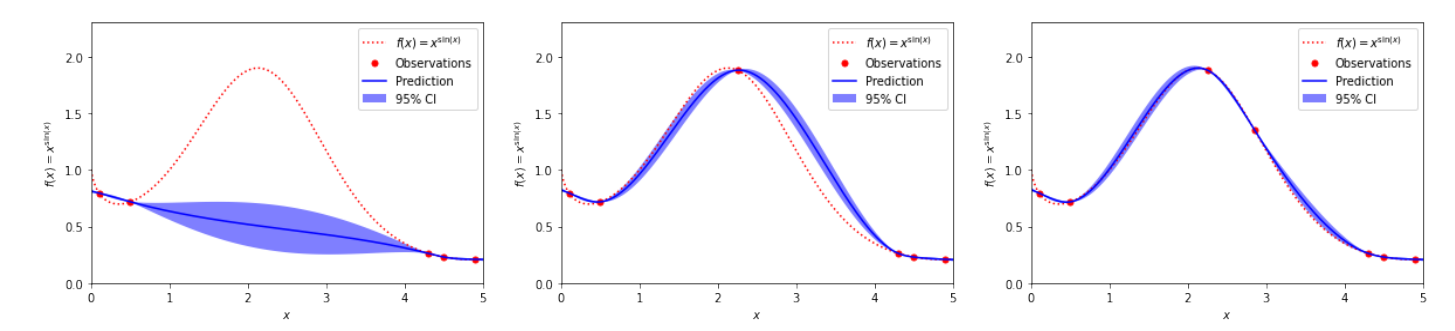
\includegraphics[width=\linewidth]{bal.png}
\end{columns}
\end{frame}

% ============================================================================
% SECTION V: RESULTS
% ============================================================================
\section{Results}

% --- Frame 30: Section Divider ---
\begin{frame}{}
\vfill
\begin{center}
{\Huge \textcolor{uzhblue}{\textbf{Part V}}}\\[12pt]
{\LARGE Results}
\end{center}
\vfill
\end{frame}

% --- Frame 31: BAU scenario ---
\begin{frame}{Business-As-Usual (BAU) Scenario}
\begin{center}
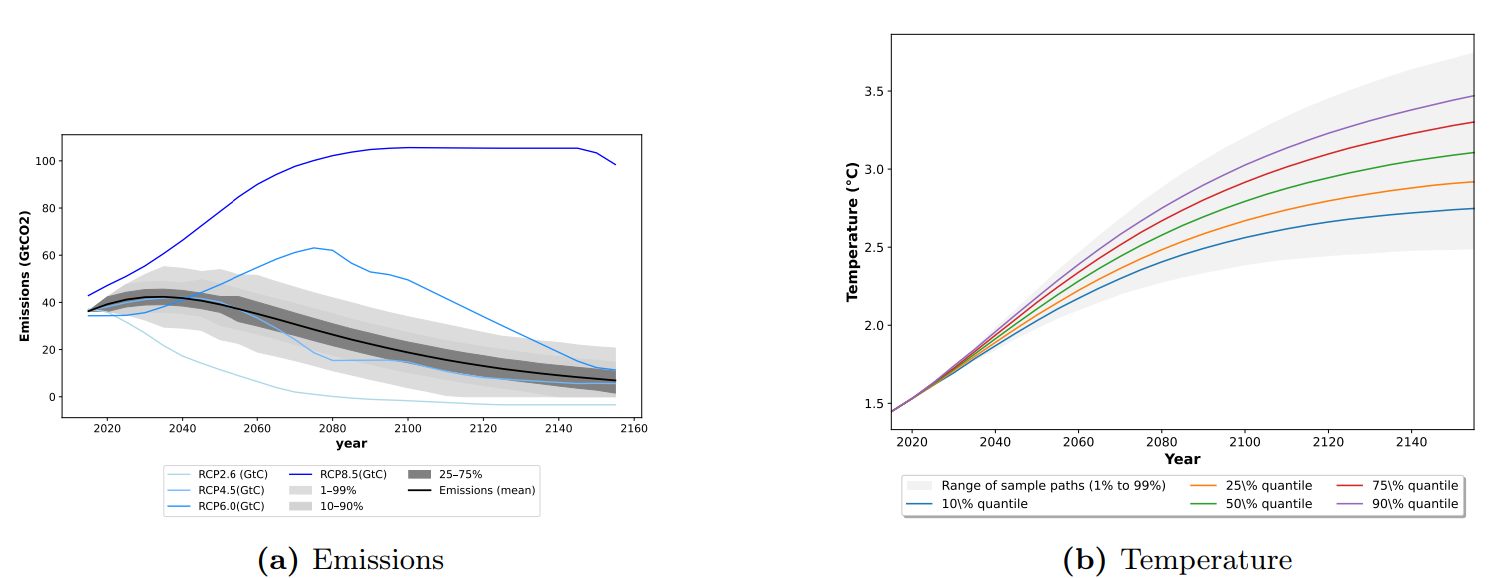
\includegraphics[width=0.78\textwidth]{BAU_SOLG.png}
\end{center}

\vspace{0.1cm}
\footnotesize
Emissions and temperature paths under no climate policy, compared with RCP scenarios.
\end{frame}

% --- Frame 32: Welfare surface ---
\begin{frame}{Welfare Surrogate Surface (Scenario 1)}
\begin{columns}[T]
\column{0.55\textwidth}
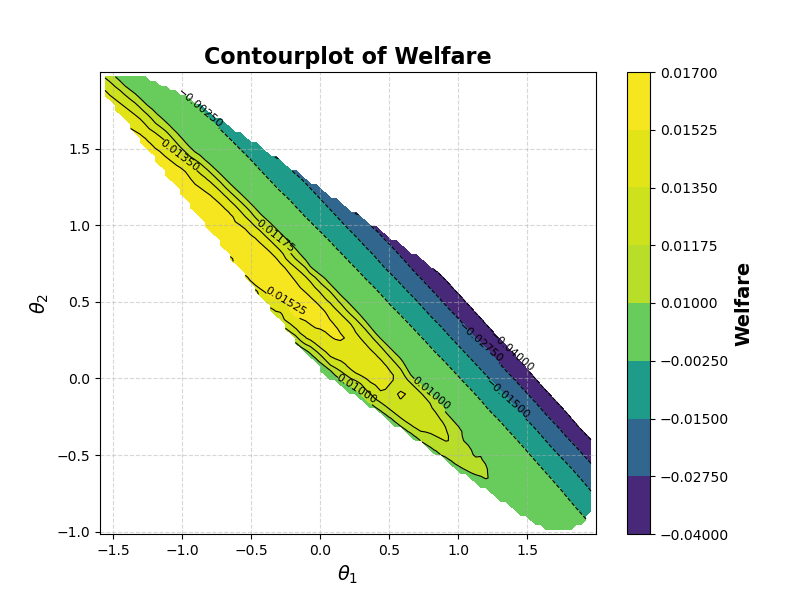
\includegraphics[width=\linewidth]{contour_welfare_E.png}

\column{0.42\textwidth}
\small
\begin{itemize}
    \item Objective surface in $(\vartheta_0, \vartheta_E)$ from GP surrogate.
    \item Smooth structure enables efficient constrained optimization.
    \item The unconstrained optimum is easy to identify but is \emphc{not Pareto-feasible}.
\end{itemize}
\end{columns}
\end{frame}

% --- Frame 33: Scenario 1 results ---
\begin{frame}{Scenario 1: Unconstrained Optimal Tax}
\begin{columns}[T]
\column{0.48\textwidth}
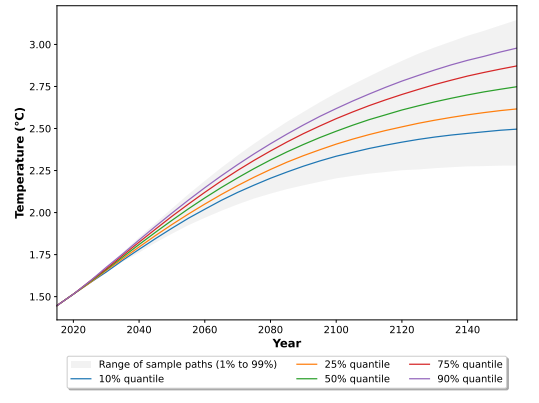
\includegraphics[width=\linewidth]{Temp_case1.png}

\column{0.48\textwidth}
\small
\begin{itemize}
    \item Strong emission reduction.
    \item Significant warming reduction.
    \item \emphc{But}: creates losers among current cohorts.
    \item Welfare losses up to $\sim$5\% for transition generations.
    \item Politically fragile without compensation.
\end{itemize}
\end{columns}
\end{frame}

% --- Frame 34: Scenario 2 --- Pareto frontier ---
\begin{frame}{Scenario 2: Pareto-Improving Policy}
\begin{columns}[T]
\column{0.48\textwidth}
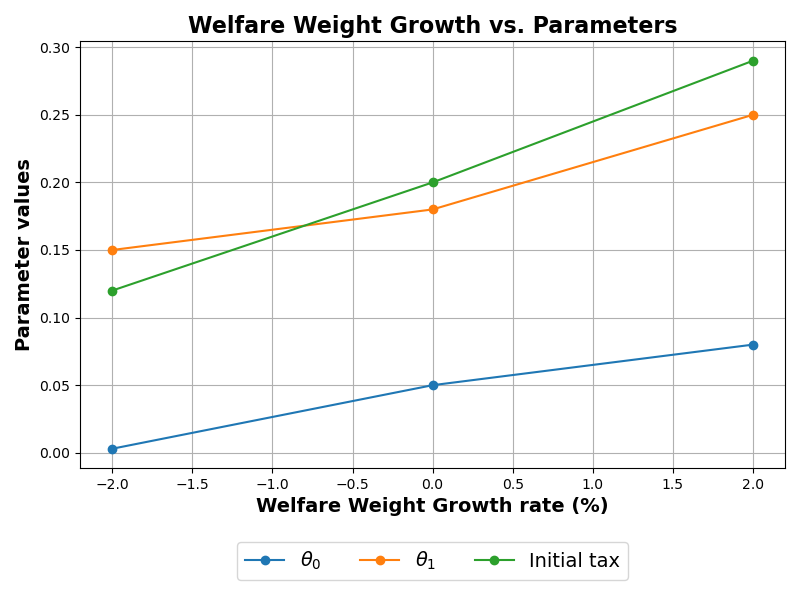
\includegraphics[width=\linewidth]{pareto_frontier_lin_E.png}

\column{0.48\textwidth}
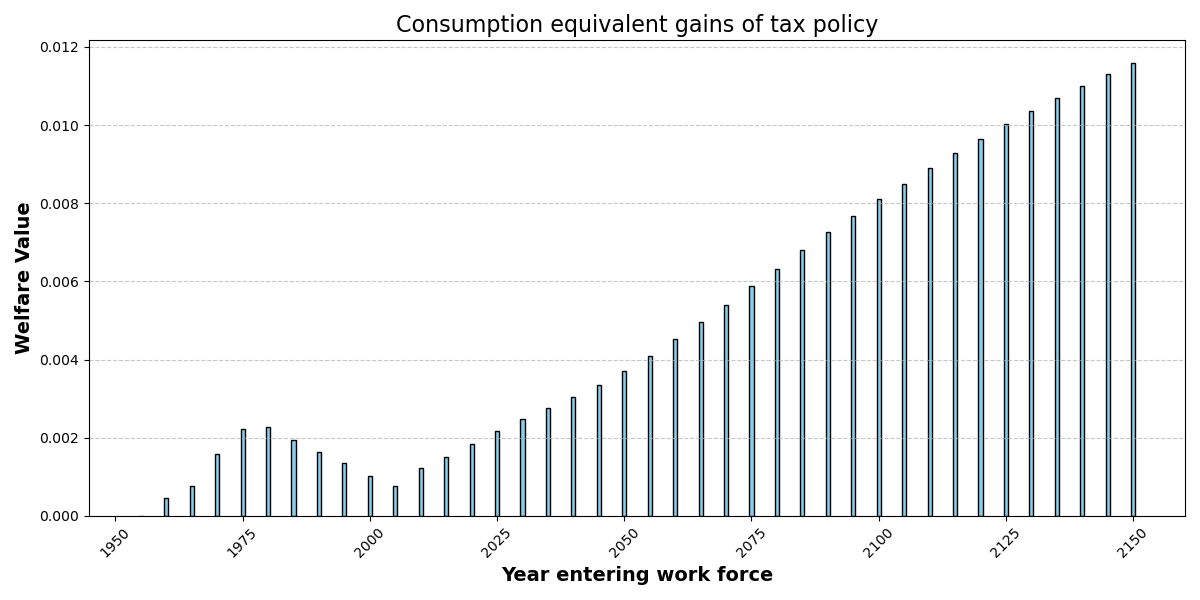
\includegraphics[width=\linewidth]{welfare_gains_pareto_S.png}
\end{columns}

\vspace{0.15cm}
\footnotesize
Left: Pareto frontier in $(\vartheta_0, \vartheta_E)$-space. Right: welfare gains by cohort --- \emphc{all non-negative} under Pareto-improving policy.
\end{frame}

% --- Frame 35: Scenario 2 --- emissions ---
\begin{frame}{Pareto Policy as Emissions-Tail Insurance}
\begin{columns}[T]
\column{0.48\textwidth}
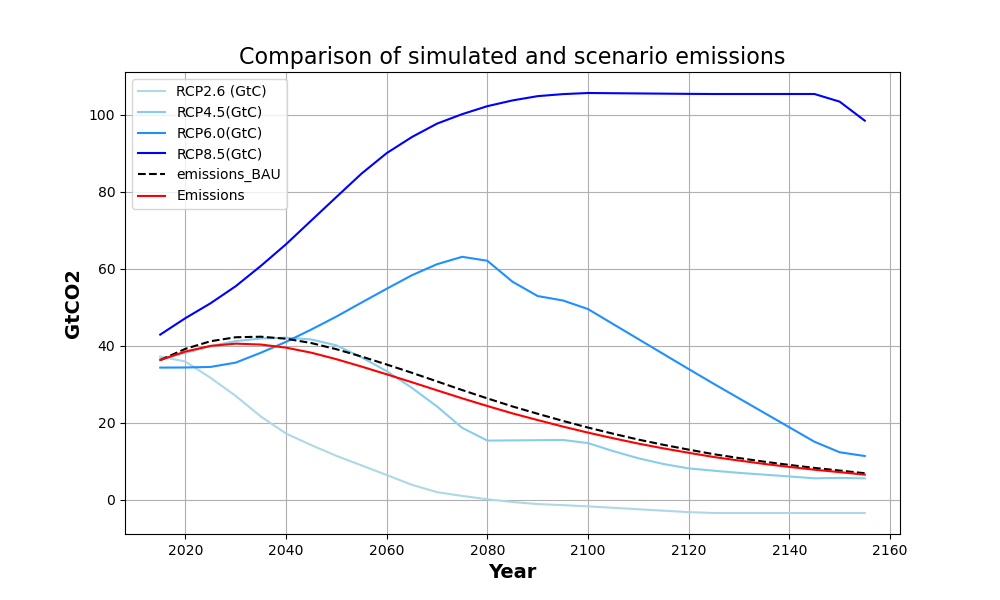
\includegraphics[width=\linewidth]{av_emissions_pareto_E.png}

\column{0.48\textwidth}
\small
\begin{itemize}
    \item Mean emissions move moderately.
    \item Upper-tail emissions are compressed materially.
    \item Main mechanism: \emphc{disaster-risk reduction} (tail insurance), not maximal average abatement.
\end{itemize}

\vspace{0.2cm}
\begin{exampleblock}{Insight}
Transfers preserve non-negative welfare effects for transition cohorts while truncating high-temperature tails.
\end{exampleblock}
\end{columns}
\end{frame}

% --- Frame 36: Scenario 3 ---
\begin{frame}{Scenario 3: Richer Tax Function}
\begin{center}
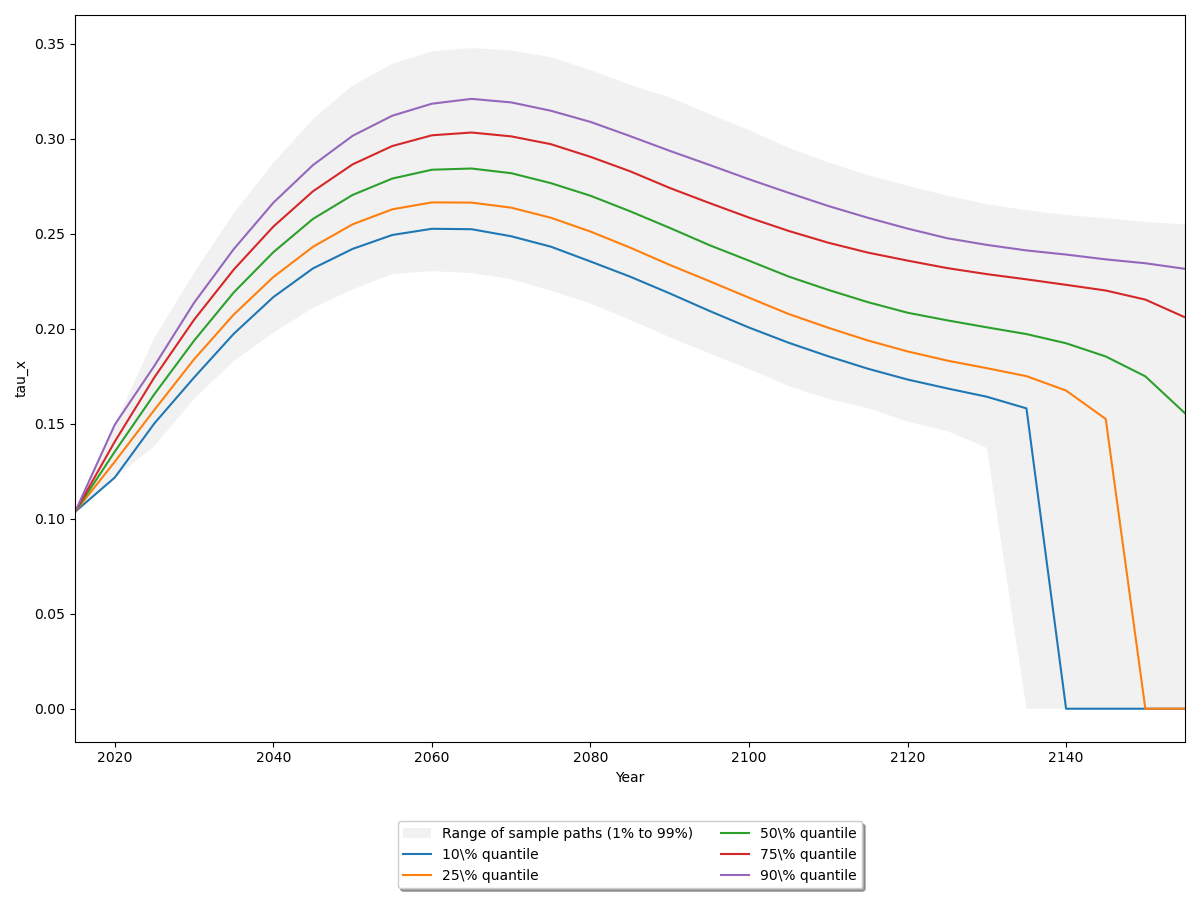
\includegraphics[height=0.55\textheight,keepaspectratio]{optimal_tax_simulation_E_kappa_tp.png}
\end{center}

\vspace{0.05cm}
\footnotesize
$\tau_t = \vartheta_0 + \vartheta_E E_t + \vartheta_\kappa \kappa_t + \vartheta_{TP}(1-D_{TP})$:
the tax responds to carbon intensity and tipping proximity, providing tipping-risk insurance.
\end{frame}

% --- Frame 37: Key economic insight ---
\begin{frame}{The Key Economic Insight}
\begin{block}{Main result}
Pareto-improving policies work through \emphc{disaster-risk reduction} (tail insurance), not maximum mean abatement \\ (empirical result from K\"ubler, Scheidegger, Surbek 2025; not proven here).
\end{block}

\vspace{0.3cm}
\begin{columns}[T]
\column{0.49\textwidth}
\textbf{What the method delivers}
\begin{itemize}
    \item Globally optimal constrained policies
    \item Transparent, implementable tax rules
    \item Welfare decomposition by cohort
    \item Sensitivity to model parameters
\end{itemize}

\column{0.49\textwidth}
\textbf{What drives the result}
\begin{itemize}
    \item Transfer design resolves intergenerational conflict
    \item Linear rules capture most of the welfare gain
    \item Richer rules add tipping-risk insurance
    \item Simple rules are robust and interpretable
\end{itemize}
\end{columns}
\end{frame}

% --- Frame 38: Key takeaways ---
\begin{frame}{Key Takeaways from Lecture 09}
\begin{enumerate}
    \item \textbf{OLG climate models are tractable with DEQNs}: 12 generations + climate + stochastic tipping solved globally.
    \item \textbf{Pseudo-states enable policy search}: tax parameters + transfer shares as inputs $\rightarrow$ solve once, optimize everywhere.
    \item \textbf{Pareto-improving policies are computationally feasible}: GP surrogate + constrained optimization in minutes.
    \item \textbf{Time as state is essential}: nonstationary dynamics (carbon intensity, abatement costs) require $t$ in the neural net input.
    \item \textbf{Tail insurance, not mean abatement}: the main welfare channel of constrained optimal policy.
\end{enumerate}

\vspace{0.2cm}
\begin{block}{Next}
Final wrap-up: course synthesis, decision guide, and research frontier.
\end{block}
\end{frame}

% --- Frame 38b: Notebook roadmap ---
\begin{frame}{Notebook Roadmap for Lecture 09}
\small
The slides here build on the deterministic CDICE-DEQN solver developed in Lecture 08; the natural notebook to revisit and extend is:
\vspace{0.2cm}
\begin{itemize}
    \item \texttt{lectures/day8/code/03\_Stochastic\_DICE\_DEQN.ipynb} -- adds an AR(1) productivity shock to the Lecture-08 deterministic CDICE-DEQN, evaluates the Euler expectation with Gauss--Hermite quadrature, and produces the SCC fan charts that motivate today's UQ discussion (parameter, stochastic, and epistemic uncertainty).
\end{itemize}
\vspace{0.2cm}
The full OLG-IAM with constrained Pareto-improving tax rules (K\"ubler, Scheidegger, Surbek 2025, arXiv:2507.01704) is implemented in production code that is not part of the classroom repository.  The paper is in the readings folder (\texttt{JPE\_Macro.pdf}); the classroom notebook focuses on the upstream stochastic CDICE-DEQN building block.
\end{frame}

% --- Frame 39: References ---
\begin{frame}{References and Reading Guide}
\small
\textbf{Core references for this lecture}
\begin{itemize}
    \item K\"ubler, Scheidegger, Surbek (2025). \emph{Using Machine Learning to Compute Constrained Optimal Carbon Tax Rules.} arXiv:2507.01704.
    \item Kotlikoff, Kubler, Polbin, Sachs, Scheidegger (2021): OLG with carbon-risk taxation.
    \item Dietz (2024), van der Ploeg and Rezai (2026), Hassler, Krusell, Smith (2016): broader climate-economics background.
    \item Azinovic, Gaegauf, Scheidegger (2022): DEQN methodology.
    \item Rasmussen and Williams (2006): Gaussian processes.
\end{itemize}

\vspace{0.25cm}
\textbf{File in this repository}
\begin{itemize}
    \item \texttt{lectures/day8/readings/JPE\_Macro.pdf}
\end{itemize}

\vspace{0.3cm}
\begin{center}
{\LARGE \emphc{Questions before wrap-up?}}
\end{center}
\end{frame}

\end{document}
